\documentclass[twocolumn]{NobArticle}
\runninghead{Autonomous Drone Swarms with IFF and Targeting}
\footertext{\textit{Rolando L. Innamorati} (2025)}

\title{Decentralized Learning for Autonomous Kamikaze Drone Swarms with Integrated IFF and Target Engagement in Adversarial Environments}

\author{
    Rolando Licia Innamorati\textsuperscript{1,2}
}

\date{
    \textsuperscript{\textbf{1}}
    Delta Service Srl
    \textsuperscript{\textbf{2}}
    Università degli Studi dell'Aquila
}

\renewcommand{\maketitlehookd}{
\begin{abstract}
    \noindent We present an integrated and decentralized learning framework for autonomous kamikaze drones equipped with friend-or-foe (IFF) classification, onboard autopilot, and swarm-level coordination. Designed for deployment on resource-constrained hardware, our system leverages end-to-end deep reinforcement learning (DRL) to train each drone to execute high-speed, collision-aware attack trajectories against mobile adversarial targets, while explicitly avoiding friendly units. Each agent operates using only local observations—including its own motion state, relative positions of nearby agents, and IFF-informed target classification—without any centralized control or global state synchronization.

    Our simulation environment models sacrificial drone behavior: upon successful impact, the agent is removed from the mission space. We define a composite reward function that promotes successful hits, penalizes collisions with teammates or friendly entities, and encourages cooperative interception patterns. Experimental results show that intelligent group behaviors such as wave-based attacks, multi-angle encirclement, and selective avoidance of non-hostile targets emerge naturally from decentralized training. This demonstrates the feasibility of building self-organizing kamikaze swarms capable of friend-aware target engagement using lightweight onboard computation, laying the groundwork for practical implementation on minimalist UAV platforms.
    \medskip

    \small{\textbf{Index Terms:} Autonomous UAVs, Kamikaze Drone, Deep Reinforcement Learning, Friend-or-Foe Recognition, Swarm Warfare.}
\end{abstract}
}

\begin{document}

\small
\maketitle

% Introduction
\section{Introduction}
    Unmanned aerial vehicle (UAV) swarms are increasingly recognized as a transformative asset in modern warfare, offering scalability, redundancy, and robustness in adversarial scenarios. When coordinated effectively, drone swarms can perform tasks ranging from area denial to reconnaissance and targeted elimination, often outperforming single-agent systems in dynamic and communication-denied environments. However, traditional approaches to multi-agent coordination typically rely on centralized planning, high-bandwidth communication, or full-state awareness, which become unreliable under electronic warfare conditions and do not scale efficiently with swarm size.
    \medskip
% Problem Definition
\section{Problem Definition}
    We consider a team of \( N \) autonomous quadrotor drones operating in a 3D simulated adversarial environment, tasked with identifying and intercepting a designated hostile target through coordinated kamikaze-style maneuvers. Each drone operates under a decentralized control policy and limited onboard sensing, with no access to global state or centralized planner. The objective is to maximize the swarm's cumulative attack effectiveness—i.e., the number and quality of successful impacts on enemy targets—while minimizing friendly-fire incidents and inefficient maneuvers.
    \medskip

    The environment is episodic, and from the global simulator perspective, the full state at time \( t \) is defined as:
    \[
    S(t) = \{s_i(t)\}_{i=1}^N \cup g(t)
    \]
    where \( s_i(t) \) is the full state of drone \( i \), and \( g(t) \) is the state of the moving adversarial target.
    \medskip

    Each agent observes only partial, local information \( o_i(t) \), which includes:
    - its own proprioceptive state \( s_i^{\text{local}}(t) \): position, velocity, orientation;
    - relative positions and velocities of up to \( K \) nearby drones;
    - the relative position of the target;
    - a binary IFF (Identification Friend or Foe) signal associated with the perceived target.
    \medskip

    Each drone \( i \) is controlled by a stochastic policy \( \pi_\theta(a_i(t) | o_i(t)) \), parameterized by a shared neural network. The action \( a_i(t) \in \mathbb{R}^4 \) corresponds to thrust commands for the quadrotor motors, producing movement according to simulated flight dynamics.
    \medskip

    Upon impact with a hostile target, the drone is considered “sacrificed” and removed from the environment. The reward function is designed to:
    - assign a large positive reward for successful impact with a hostile target;
    - penalize collisions with teammates or friendly-classified targets;
    - reward proximity to the target to guide learning during early training.
    \medskip

    The episode terminates when all drones are either sacrificed or the maximum time horizon \( T \) is reached.
    \medskip

    This formulation enables the study of self-organizing kamikaze strategies, IFF-informed target discrimination, and emergent multi-agent coordination under decentralized control and limited perception.
    \medskip
% Methodology
\section{Methodology}

% Experimental Evaluation
\section{Experimental Evaluation}

    \subsection{First Steps}
        As a natural continuation of the methodological design, the experimental evaluation began with a deliberately simplified implementation. Our intention at this stage was not to prove the final effectiveness of the system, but rather to verify that the pipeline---from simulation environment to training and logging, and finally to analysis and visualization---was functioning in practice. To do this, we chose to start with a two-dimensional environment. This decision was motivated by two main reasons: on the one hand, it drastically reduces computational and implementation complexity compared to a full 3D quadrotor simulation; on the other hand, it allows much faster iteration cycles, enabling us to quickly observe whether the learning dynamics of the swarm produced any coherent behavior or if everything remained random noise. In other words, the 2D environment represented the most direct way to put the theoretical framework to the test and obtain immediate feedback.
        \medskip

    \subsection{Setup (Common Across P0--P1)}
        We consider a planar interception task in discrete time $t=0,1,\dots$, where a drone agent must reach a fixed target. The agent observes a normalized state vector
        \begin{equation}
            \label{eq:obs}
            \mathbf{o}_t \;=\; \frac{1}{\max(1,\,\texttt{plane}-1)}\,[\,x_t,\,y_t,\,x^{(\mathrm{tar})},\,y^{(\mathrm{tar})}\,] \in [0,1]^4,
        \end{equation}
        with $(x_t,y_t)$ the drone cell and $(x^{(\mathrm{tar})},y^{(\mathrm{tar})})$ the target cell.\footnote{Normalization as implemented in \texttt{\_norm\_obs}, denominator $\max(1,\texttt{plane}-1)$.}
        \medskip

        At each step, the agent selects a discrete action $a_t\in\mathcal{A}$ that moves the drone by a displacement $(\Delta x,\Delta y)$ clipped within the arena bounds; next state, Euclidean distance $d_t$, and termination are computed accordingly.\footnote{Environment step: integer grid move, clamped to $[0,\texttt{plane}-1]$, with termination on $d_t\le\varepsilon$ or $t\ge\texttt{MAX\_STEPS}$.}

        \subsubsection{Reward shaping.}
            Let $d_t$ be the Euclidean drone–target distance and $d_{\max}=\sqrt{2}\,(\texttt{plane}-1)$ the maximum diagonal distance. The per-step reward is
            \begin{align}
                r_t \;=\; &\underbrace{K \big(\tfrac{d_{t-1}}{d_{\max}}-\tfrac{d_t}{d_{\max}}\big)}_{\text{progress (normalized)}} \;-\; \underbrace{c_{\mathrm{step}}}_{\text{step cost}}
                \;-\; \underbrace{c_{\mathrm{turn}}\,[a_t\neq a_{t-1}]}_{\text{turn penalty}}
                \;-\; \underbrace{c_{\mathrm{rev}}\,[s_t\in\mathcal{V}]}_{\text{revisit penalty}}, \label{eq:reward}\\
                &\text{plus terminal terms:}\quad
                \begin{cases}
                +R\,(1+\tfrac{T_{\max}-t}{T_{\max}}) & \text{if } d_t\le \varepsilon \\
                - R_{\mathrm{to}} & \text{if } t\!=\!T_{\max}
                \end{cases}\nonumber
            \end{align}
            with $K=1.0$, $c_{\mathrm{step}}{=}0.003$, $c_{\mathrm{turn}}{=}0.002$, $c_{\mathrm{rev}}{=}0.01$, $R{=}20.0$, $R_{\mathrm{to}}{=}1.0$ in the large-grid setting; the success threshold is $\varepsilon=\max(1.0,0.005\cdot \texttt{PLANE\_SIZE})$.%

            This is a potential-based shaping on $d_t$ (distance) plus small control-like regularizers.

        \subsubsection{Learning.}
            In P0--P1 we use a neural $Q$-function $Q_\theta(\mathbf{o},a)$ trained with Double DQN and a target network. The function approximator is a 2-layer MLP (256–256 ReLU) with $|\mathcal{A}|$ outputs, Huber loss, gradient clipping, and Adam optimizer.\footnote{Architecture and update: 2-layer MLP (256,256) → $|\mathcal{A}|$; Double DQN target with online $\arg\max$ and target gather; Huber loss; grad clip at 5.0; Adam with $\mathrm{lr}=1.5\mathrm{e}{-3}$.}
            Exploration is $\varepsilon$-greedy with linear decay $\varepsilon(s)$ from $0.25$ to $0.02$ over $150\text{k}$ steps; replay buffer size $3\!\times\!10^5$, batch $256$, $\gamma=0.99$, target sync every $2\text{k}$ updates.

        \subsubsection{Evaluation.}
            We report success rate ($\%$ of episodes reaching $d_t\le\varepsilon$), average return (shaped), and average steps, via a greedy policy ($\arg\max_a Q$) on uniformly random spawns over the full arena. For visualization, we use an offline \emph{play} that reproduces the same observation normalization and arena parameters (\texttt{plane}, \texttt{MAX\_STEPS}, $\varepsilon$) saved in the training checkpoint.\footnote{The playback environment uses identical normalization (Eq.~\eqref{eq:obs}) and termination to avoid train–eval mismatch.}

    \subsection{P0 — Tiny Grid (small 2D grid, 4 directions + stay)}
        \subsubsection{Objective.}
            Sanity-check the full pipeline (environment, reward shaping, logging, evaluation) and verify that the learned policy develops a consistent homing behavior on a small grid with $|\mathcal{A}|=5$ (N/S/E/W + stay).

        \subsubsection{Methodology.}
            Same $Q_\theta$ architecture (smaller action set). Reward shaping as in Eq.~\eqref{eq:reward} with the same structure; smaller arena implies a larger per-step progress signal $\Delta d/d_{\max}$ and naturally easier credit assignment.

        \subsubsection{Results.}
            Across seeds, training curves show a monotonic rise in success with diminishing variance; representative windows reached $\approx 70\%\!\to\!90\%$ success as training proceeds (consistent with step-wise shaped returns improving over time). Qualitative rollouts show direct, low-zigzag homing; near-target corrections are mild due to the small $c_{\mathrm{turn}}$ and the positive progress term.

        \subsubsection{Takeaways.}
            The shaping in Eq.~\eqref{eq:reward} is sufficient to break symmetry and converge quickly on small grids; the observation normalization in Eq.~\eqref{eq:obs} prevents scale issues and enables reuse on larger arenas.

    \subsection{P1 — Big Grid DQN (101$\times$101, 8 directions + stay)}
        \subsubsection{Objective.}
            Scale to a larger arena (\texttt{PLANE\_SIZE}$=101$), expand the action set to 8 compass moves + stay ($|\mathcal{A}|=9$), and validate stability of Double DQN under sparse terminal rewards.

        \subsubsection{Curriculum on spawn distance.}
            To unlock early successes and propagate terminal value, we constrain the initial Manhattan distance $\|p_0 - p_0^{(\mathrm{tar})}\|_1 \le D_{\max}(e)$ with a schedule
            \[
            D_{\max}(e)=
            \begin{cases}
            20,& e<500\\
            40,& 500\le e<2000\\
            \texttt{PLANE\_SIZE},& e\ge 2000
            \end{cases}
            \]
            where $e$ is the episode index; beyond $e\!\ge\!2000$ we use full-arena spawns.\footnote{Spawn curriculum implemented in \texttt{reset(episode)} with \texttt{max\_spawn\_manhattan\_for\_episode}.}

        \subsubsection{Reward calibration.}
            On a $101\times 101$ grid the unit progress is $\Delta d/d_{\max}\approx 1/\sqrt{2}\,(\texttt{plane}-1)^{-1}\approx 0.007$, hence we lower $c_{\mathrm{turn}}$ to $0.002$ and $c_{\mathrm{step}}$ to $0.003$ so that a single correct move near the target remains net-positive; the arrival bonus $R{=}20$ ensures rare successes dominate return and backpropagate through bootstrapping.\footnote{Large-grid constants used: $c_{\mathrm{turn}}{=}0.002$, $c_{\mathrm{step}}{=}0.003$, $R{=}20$.}

        \subsubsection{Training configuration.}
            We train for up to $1000$ episodes with replay $3\!\times\!10^5$, batch 256, $\gamma=0.99$, Adam ($1.5\!\times\!10^{-3}$), target sync every $2000$ updates, $\varepsilon$-greedy from $0.25$ to $0.02$ over $150$k steps, gradient clip $5.0$.
            The observation normalization, termination, and evaluation are identical to training to avoid distribution shift.

        \subsubsection{Metrics and representative outcome.}
            We monitor success rate, shaped average return, and average steps. In a representative large-grid run, the training summary reported
            \emph{[Ep 1000] avg\_return = 39.116, $\varepsilon=0.101$, success\_rate = 87.80\%}.%
            % (User-provided log)
            Qualitatively, evaluation rollouts (pure $\arg\max$) reach the target without orbiting; the reduction of $c_{\mathrm{turn}}$ removes pathological near-target zigzag and improves closure.

            \begin{figure}[H]
                \centering
                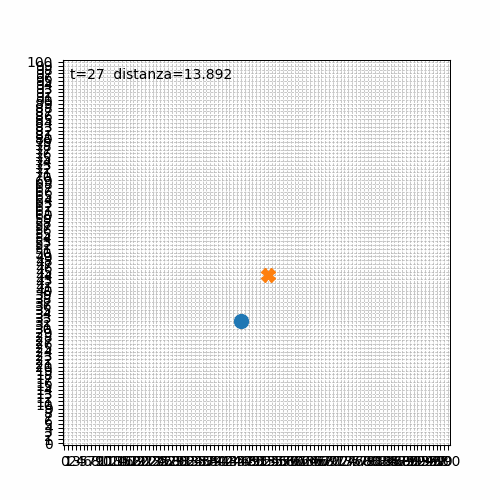
\includegraphics[scale=0.5]{Figures/step_2_t2.png}
                \caption{Representative greedy rollout on the large grid (P1). The agent closes on the target with minimal zigzag. Animated version can be found on our \underline{\href{https://github.com/rolandoinnamorati/swarm-rl}{GitHub repository.}}}
            \end{figure}

% Related Works
\section{Related Works}
    Research on autonomous unmanned aerial vehicle (UAV) swarms has progressed significantly in recent years, particularly in the context of distributed control, coordinated behavior, and intelligent targeting. Our work draws inspiration from three main lines of prior research: decentralized learning for multi-agent swarms, embedded kamikaze UAV systems, and artificial intelligence methods for friend-or-foe (IFF) classification.
    \medskip

    \cite{batra2022decentralized} demonstrated the feasibility of learning decentralized swarm behaviors via end-to-end deep reinforcement learning (DRL), enabling individual quadrotors to navigate, avoid collisions, and maintain formation in fully simulated environments. Their framework required only local observations and showed successful sim-to-real transfer on resource-constrained quadrotor platforms. However, their work was limited to general flocking and pursuit-evasion tasks, without addressing targeting logic, engagement, or threat discrimination. In contrast, our work focuses specifically on offensive kamikaze-style behaviors, integrated with IFF and attack coordination under tactical constraints.
    \medskip

    On the hardware and systems side, \cite{muda2024kamikaze} presented a physical implementation of a kamikaze drone built around the ESP32 microcontroller. Their prototype combined a GPS-guided autopilot, PID flight stabilization, and simple onboard target recognition based on distance and color segmentation. While effective for linear, single-drone attack missions, the system lacked dynamic swarm behavior and did not incorporate any learning-based adaptability or multi-agent strategy. Our approach complements this by focusing on swarm-level intelligence and decentralized coordination, which could be integrated with similar lightweight hardware platforms.
    \medskip

    Finally, the work \cite{rachman2024enemy} on IFF-based enemy detection proposes the use of neural networks trained on electromagnetic signatures to classify detected entities as friend or foe. Their AI-based model aims to support ethical engagement by reducing the risk of fratricide in autonomous operations. This concern directly aligns with our inclusion of IFF-like discrimination in the agent observation space and reward function. We build upon this by embedding such logic into reinforcement learning policies, enabling drones to not only detect but react to friendly or hostile classifications during swarm missions.
    \medskip

    Together, these works provide the foundation for our integrated framework, which unites DRL-based swarm coordination, kamikaze mission profiles, and AI-driven IFF mechanisms into a single, deployable decision-making system for offensive UAV swarms operating in adversarial environments.

% Ethical Considerations
\section{Ethical Considerations}
    The development of autonomous weapon systems, including kamikaze drone swarms, raises significant ethical concerns related to accountability, reliability, safety, and compliance with international humanitarian law. While the present study is conducted entirely in simulation and remains within the scope of academic exploration, the underlying capabilities—autonomous target interception, decentralized decision-making, and friend-or-foe discrimination—intersect with real-world domains where lives may be at stake.
    \medskip

    A core concern involves the use of machine learning for lethal decision-making. In our system, drones are trained to autonomously select and engage targets based on onboard observations and IFF classification. Misclassification or model misbehavior could result in friendly fire incidents or unlawful engagements. These risks are exacerbated by the black-box nature of neural policies and the lack of human oversight in decentralized execution.
    \medskip

    Moreover, the kamikaze paradigm by design removes the possibility of post-engagement correction. Once launched, a drone that misidentifies its target cannot be recalled. This necessitates an extremely high standard of robustness, explainability, and fail-safety—none of which current DRL models fully guarantee.
    \medskip

    In light of this, future real-world implementations must integrate comprehensive safety mechanisms, including human-in-the-loop or human-on-the-loop protocols, formal verification of critical components, and externally enforced abort or override systems. Ethical deployment also requires adherence to the principles of necessity, proportionality, and distinction as articulated in the laws of armed conflict.
    \medskip

    While our simulation includes IFF inputs and penalizes misengagement, we emphasize that this is an abstraction. The real-world challenge of building reliable IFF modules is non-trivial and cannot be offloaded entirely to AI models. The inclusion of such mechanisms in this research should be interpreted as a placeholder for more rigorous safety architecture.
    \medskip

    We also explicitly discourage the deployment of purely autonomous lethal systems based on this or similar research without extensive ethical, legal, and operational vetting. Our goal is to explore the computational feasibility of decentralized swarm intelligence in high-stakes scenarios, not to advocate for fully unsupervised engagement models.
% Conclusion
\section{Conclusion \& Future Works}

% Appendix
\section*{Appendices}

    \subsection*{A — Glossary of Terms and Acronyms}
        \addcontentsline{toc}{subsection}{A. Glossary of Terms and Acronyms}
        \begin{itemize}
            \item \textbf{UAV} — Unmanned Aerial Vehicle; an aircraft without a human pilot onboard, commonly referred to as a drone.

            \item \textbf{DRL} — Deep Reinforcement Learning; a class of machine learning algorithms combining deep learning and reinforcement learning principles to learn policies in high-dimensional spaces.

            \item \textbf{RL} — Reinforcement Learning; a machine learning paradigm in which agents learn to take actions in an environment to maximize cumulative reward.

            \item \textbf{PPO} — Proximal Policy Optimization; a state-of-the-art policy gradient algorithm used in reinforcement learning for training stable and efficient stochastic policies.

            \item \textbf{IFF} — Identification Friend or Foe; a method for automatically distinguishing allied units from enemies, critical for avoiding fratricide in combat scenarios.

            \item \textbf{GNN} — Graph Neural Network; a type of neural network architecture particularly suited for learning over structured graph data, often applied in multi-agent systems.

            \item \textbf{PID} — Proportional-Integral-Derivative controller; a classical control algorithm widely used in robotics and flight control systems.

            \item \textbf{P2P} — Peer-to-Peer; a decentralized communication model in which nodes (e.g., drones) share information directly without a central coordinator.

            \item \textbf{ESP32} — A low-cost, low-power microcontroller with built-in Wi-Fi and Bluetooth, commonly used in lightweight embedded UAV systems.

            \item \textbf{GUI} — Graphical User Interface; a visual interface for interacting with a system, in this context referring to the visual output of the PyBullet simulator.

            \item \textbf{CNN} — Convolutional Neural Network; a deep learning architecture mainly used for processing grid-like data such as images, potentially applicable to onboard visual recognition.

            \item \textbf{RLlib} — A scalable library for reinforcement learning built on Ray, commonly used for distributed training of agents.

            \item \textbf{SB3} — Stable-Baselines3; a widely used Python library for reinforcement learning built on top of PyTorch, offering standard implementations of DRL algorithms.

            \item \textbf{LAWS} — Lethal Autonomous Weapon Systems; weapon systems that can select and engage targets without human intervention, a subject of active ethical and legal debate.

            \item \textbf{LOAC} — Law of Armed Conflict; the body of international law regulating the conduct of armed hostilities, including principles such as distinction, proportionality, and necessity.

            \item \textbf{CNN-based IFF} — An IFF system based on convolutional neural networks, used to classify visual or sensor data as friend or foe.

            \item \textbf{Sim-to-Real} — A methodology where models trained in simulation are transferred to real-world systems with minimal adjustment.

            \item \textbf{Autopilot} — A control system that allows a vehicle to operate independently by following a pre-programmed or dynamically generated trajectory.

            \item \textbf{Swarm Intelligence} — The collective behavior of decentralized, self-organized systems, often inspired by natural phenomena like bird flocks or ant colonies.

            \item \textbf{Black-box Model} — A model whose internal workings are not transparent or easily interpretable, typically referring to deep neural networks.

            \item \textbf{Reward Shaping} — A reinforcement learning technique where intermediate rewards are introduced to accelerate and guide learning.

            \item \textbf{Kill Switch} — A hardware or software mechanism that allows emergency interruption or disabling of an autonomous system.
        \end{itemize}

\printbibliography

\end{document}
